\documentclass[main.tex]{subfiles}
\begin{document}

\custompart{Quantifier l'\hetero d'une tumeur à partir d'une image}{Comment ? Par quel biais? Exploration de différents critères.}{Dans cette partie, on propose d'examiner en détail le caractère \heterogene de nos images - les images médicales ainsi que les images produites numériquement avec le modèle EDP. Dans un premier temps, nous présenterons la construction d'histogrammes des niveaux de gris contenus dans l'image. Dans un second temps, nous décrirons ces histogrammes par un mélange de gaussienne. Enfin ce mélange gaussien sera utilisé pour calculer différents critères qui seront comparés. }

\chapter{Construction des histogrammes de niveaux de gris}
\chapter{Fit des histogrammes}
\todo[noline]{On peut employer le mot "fit" ?}
\chapter{Critères quantifiant l'\hetero.}

%%http://ctan.mines-albi.fr/macros/latex/contrib/lettrine/doc/demo.pdf
\renewcommand{\LettrineFontHook}{
%\fontfamily{yfrak}
\fontfamily{pag}
\fontseries{bx}\fontshape{it}
%\color[gray]{0.5}
}
%\lettrine[lines=2, lhang=0.33, loversize=0.25]{$\mathscr{D}$}{ans} 
\lettrine[lines=2, lhang=0.33, loversize=0.25]{D}{ans} 
tout ce chapitre, on considère l'approximation en un mélange de 2 gaussiennes d'un histogramme de niveau gris. Ce mélange gaussien est entièrement décrit par les paramètres suivants:
\begin{itemize}
\item $c_1, c_2$ : Centre des gaussiennes.
%% Sans pertes de généralité on peut admettre que l'on a ordonné les gaussienne \ie $c_1<c_2$.
\item $\sigma_1,\sigma_2$ : Ecart-type de chacune des gaussiennes
\item $w_1,w_2$ : Poids associées aux gaussiennes dans le mélange ($w_1+w_2=1$)
\end{itemize}
On peut ainsi définir plusieurs quantités caractéristiques :
\begin{itemize}
\item $h_1,h_2$ : Hauteur des gaussiennes. Elles sont données par $h_i = \frac{w_i}{\sigma_i\sqrt{2\pi}}$
\end{itemize}
Notons $\Delta$ l'opérateur de différence défini par :
\begin{equation}
\label{eq:operateur_delta_gaussienne}
\Delta :  u \longmapsto \Delta u := u_2 - u_1.
\end{equation}
Ainsi les quantités suivantes pourront s'avérée intéressantes à étudier : $\Delta c$, $\Delta \sigma$,  $\Delta \sigma^2$, $\Delta h$, $\Delta w$ représentant respectivement l'écart entre les centres, la différence d'écart-type, la différence des variances, la différence des hauteurs et la diffirences des poids. On pourra aussi regarder le ratio des quantités :
\begin{equation}
\label{eq:operateur_quotient_gaussienne}
Q :  u \longmapsto Qu := \dfrac{ \min( u_2 , u_1) }{ \max( u_2 , u_1)  }.
\end{equation}

Afin de correctement traduire l'\hetero, il est nécéssaire de fournir une fonction objectif que notre critère devra reproduire au mieux. Ainsi, j'ai décidé de catégoriser l'ensemble des scanners de nos patients. Le partage des scanners est ainsi fait en 5 catégories, en associant à chaque catégorie une valeur de l'\hetero $\mathscr{H}$ :
\begin{itemize}
\item $\mathscr{H}=0.9$ : très \heterogene
\item $\mathscr{H}=0.7$ : plutôt \heterogene
\item $\mathscr{H}=0.5$ : cas intermédiaire ou difficile à caractériser
\item $\mathscr{H}=0.3$ : plutôt homogène
\item  $\mathscr{H}=0.1$ : très homogène
\end{itemize}
Après appréciation visuelle \footnote{\samepage Cette appréciation visuelle reste ma perception personnelle même si je me suis efforcer de rester le plus objectif possible. Mettre à contribution les membres de l'équipe de recherche par exemple, pour leur demander une catégorisation aurait pu permettre de confronter l'évolution de l'\hetero au cours du temps que je perçois à celle que perçoivent les autres. La fonction objectif finale pourrait ainsi être la moyenne de celles que chacun obtient. On aurait donc un peu plus de nuances : des valeurs intermédiaires aux 5 paliers notamment ainsi que des barres d'erreur pour chaque valeur}
%(la fonction objectif sera appelée \hetero visuelle)
, voici ce que donne les fonctions objectifs pour $\mathscr{H}$ (cf. Fig. \ref{fig:hetero_visuelle} ).

\begin{figure}
\subfloat[\label{fig:hetero_objectif_Nber}\Nber]{\includegraphics[width=0.48\textwidth]{graph_hetero/dcm_Nber/00-note_hetero.png}}
\subfloat[\label{fig:hetero_objectif_Chen}\Chen]{\includegraphics[width=0.48\textwidth]{graph_hetero/dcm_Chen/00-note_hetero.png}}
\caption{\label{fig:hetero_visuelle}Fonction objectif de l'\hetero}
\end{figure}

Notons que \Nber est encore ici un cas très représentatif de ce que l'on cherche à étudier \ie corrélation entre \hetero et rechute imminente. En effet, ici l'\hetero croit avant même que le volume tumorale ne réaugmente, signe de la reprise d'activité cellulaire sur le pourtour de la métastase. Le coeur reste nécrosé et donc l'\hetero est accrue. Lorsque le volume tumorale fini par augmenter, le tissu proliférant à, en grande partie (si le centre de la tumeur est suffisament vascularisé), recoloniser la zone nécrosée. La croissance de la métastase est alors synonyme d'homogénéisation, puisque l'ensemble de la surface tumorale tend à être proliférante. Une homogénéisation a également lieu lorsque le traitement est efficace. Dans ce cas-ci, l'ensemble de la tumeur tend à être nécrosée.

Examinons à présent, les informations que fournissent les quantités suivantes (qui pourraient être des quantificateurs de l'\hetero):
\begin{align}
\mathcal{H}_1 =& \frac{|\Delta c |}{256}, \\
\mathcal{H}'_1 =& 1-Qc \\ %%1-\frac{ \min(c_1,c_2) }{\max(c_1,c_2)}, \\
\mathcal{H}'_2 =& \left| \frac{\Delta c / 256 }{\Delta h}\right|, \\
%% \mathsrc{A} & %%% on ne peut pas utiliser mathsrc ici ...
\mathcal{H}_3 =& Qw, \\ %%\frac{ \min (w_1,w_2) }{ \max (w_1,w_2) },  
\\
\mathcal{H}'_3 =& |\Delta w|, \\
\mathcal{H}_8 =& |\Delta h|, \\
\mathcal{H}'_8 =& \frac{ \min (h_1,h_2) }{ \max (h_1,h_2) },
\end{align}

\begin{figure}[htpb]
\subfloat[\label{fig:critere_dc}Critères basés sur $\Delta c$]{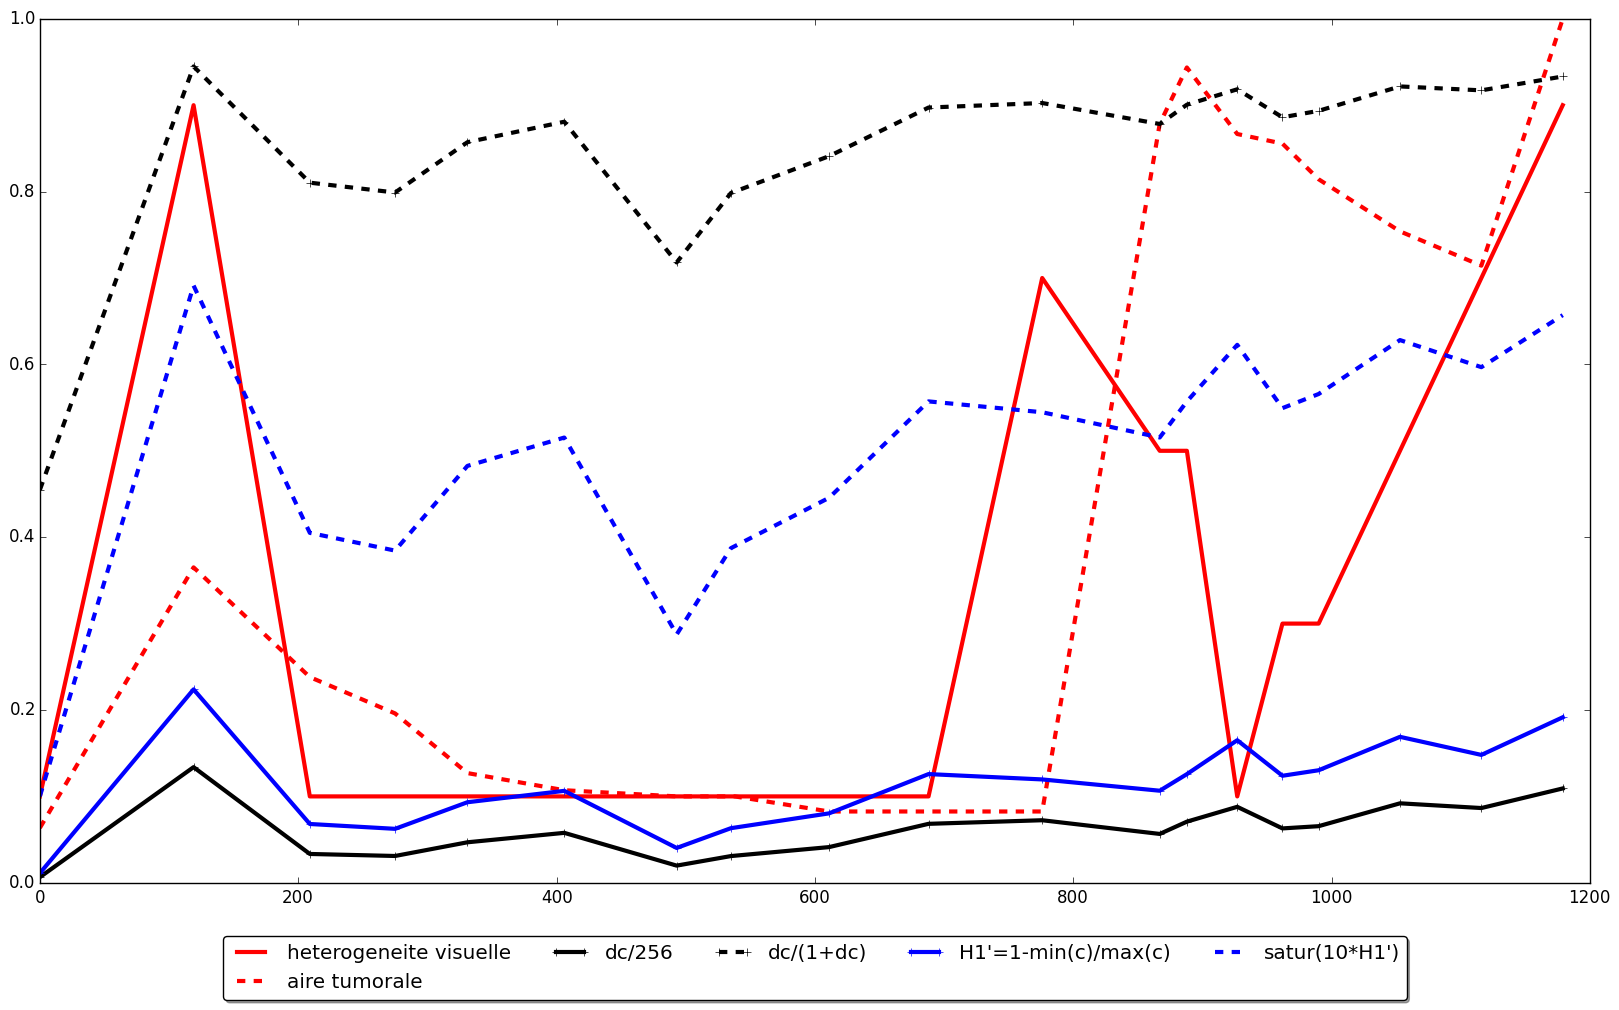
\includegraphics[width=0.48\textwidth]{graph_hetero/dcm_Nber/01-dc.png}}
\subfloat[\label{fig:critere_dh}Critères basés sur $\Delta h$]{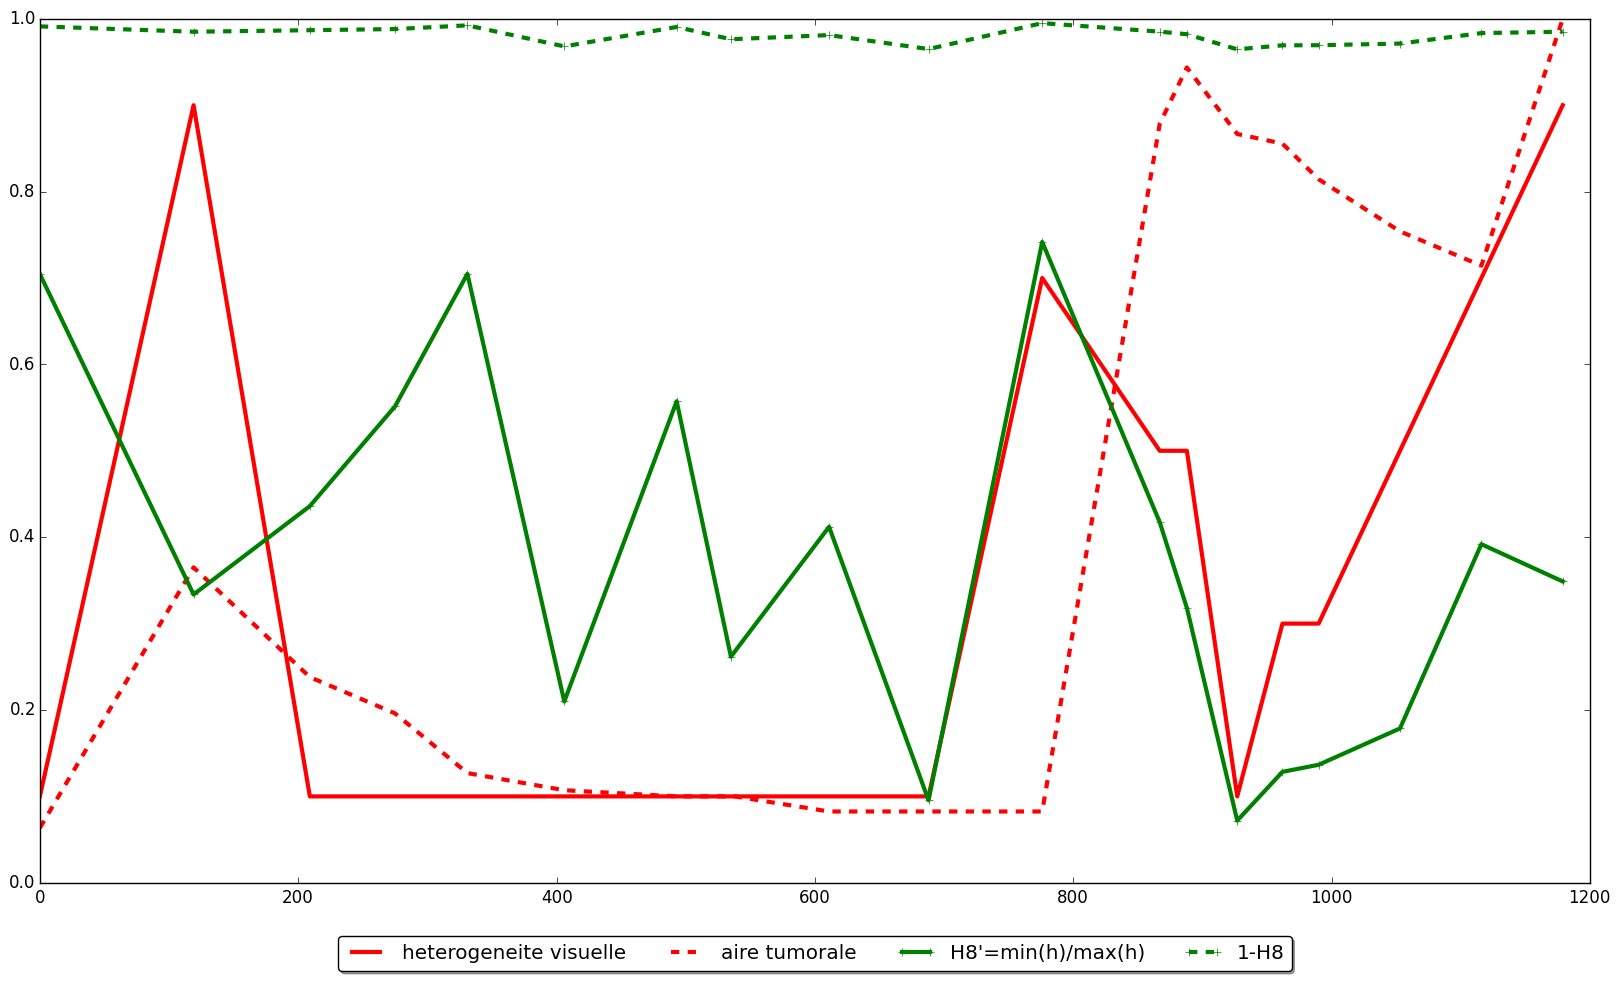
\includegraphics[width=0.48\textwidth]{graph_hetero/dcm_Nber/02-dh.png}}
\\
\centering
\subfloat[\label{fig:critere_dw}Critères basés sur $\Delta w$]{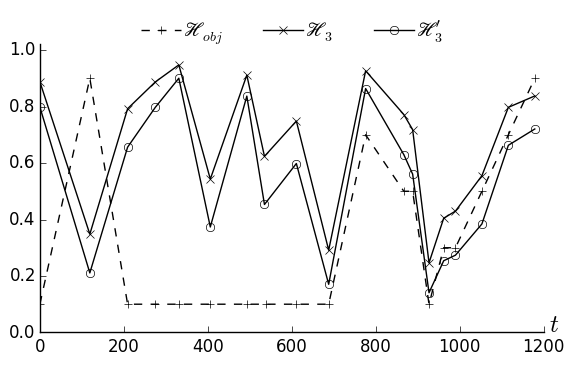
\includegraphics[width=0.48\textwidth]{graph_hetero/dcm_Nber/02_2-dw.png}}
\caption{\label{fig:premiers_criteres}Premiers critères}
\end{figure}
\begin{figure}[htpb]
\centering
%\subfloat[\label{fig:critere_dc_sur_dh}Critères basés sur la pente $\dfrac{\Delta c}{\Delta h}$]{
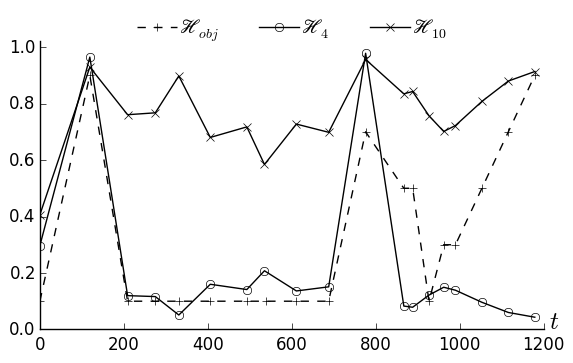
\includegraphics[width=0.70\textwidth]{graph_hetero/dcm_Nber/03-atan(dc_sur_dh).png}
%}
\caption{\label{fig:critere_dc_sur_dh}Critères basés sur la pente $\Delta c / \Delta h$}
\end{figure}

La Figure \ref{fig:premiers_criteres} montre l'évolution de ces différentes quantités (ou de quantités qui en découle) au cours du temps. 
Les ratios $Qc, Qh$ et $Qw$ sont par définition entre 0 et 1. 
Notez que $\Delta h$ et $\Delta w$ sont nécessairement compris entre 0 et 1, puisqu'ils sont la différence de 2 élements compris entre ces même bornes. En ce qui concerne $\Delta c$ on le divisera par 256, pour également le ramener dans cet intervalle. Pour garantir l'appartenance à l'intervalle $[0,1]$, on pourra également saturer les quantités :
\begin{equation}
\label{eq:saturation_critere}
\mathscr{S}: x \longmapsto \dfrac{x}{1+x}
\end{equation}

On remarque qu'aucune de ces quantités n'est pertinente pour décrire l'\hetero. Outre cela, on peut également remarquer les équivalences suivantes :
\begin{equation}
\label{eq:equiv_diff_rapport}
\dfrac{\Delta c}{256} \simeq 1 - \dfrac{\min(c_1,c_2)}{\max(c_1,c_2)} \quad {\rm et } \quad \Delta w \simeq 1 - \dfrac{\min(w_1,w_2)}{\max(w_1,w_2)}.
\end{equation}
Pour $\Delta h$, on a visiblement pas d'équivalence stricte mais les variations du ratio semble être une dilatation de celles de la différence.


\end{document}